\section{移动平台}
TensorFlow对于移动平台被设计为一个好的深度学习解决方案。
当前我们已经有两个解决方案用于部署机器学习应用到移动设备和嵌入式设备:\href{https://www.tensorflow.org/mobile/mobile_intro?hl=zh-cn}{TensorFlow for Mobile}和\href{https://www.tensorflow.org/mobile/tflite/index?hl=zh-cn}{TensorFlow Lite}。
\subsection{TensorFlow LiteVS TensorFlow Mobile}
下面是两者的一些不同之处:
\begin{itemize}
\item TensorFlow Lite是TensorFlow Mobile的一个进化版本。在多属性框虾,用TensorFlow Lite开发的app二进制文件更小,依赖更小,性能更强。
\item TensorFlow Lite是在开发者预览中,因此不是所有情况都能覆盖。我们希望你用TensorFlow Mobile覆盖产品。
\item TensorFlow Lite仅仅支持有限的操作,因此不是所有的模型都能在上面运行的很好。TensorFlow Mobile对函数有一个更完整的支持。
\end{itemize}
TensorFlow Lite为移动平台提供了更好的性能和更小的文件尺寸如果在它们的平台上一些硬件加速功能加速功能可以使用的话。另外,它有更少的依赖以至于它可能被构建运行在更简单的,资源首先得设备上。TensorFlow Lite可允许通过\href{https://developer.android.com/ndk/guides/neuralnetworks/index.html?hl=zh-cn}{Neural Networks API}加速。

TensorFlow Lite当前已经覆盖了有限的一些操作。尽管默认TensorFlow Mobile支持仅仅支持有限的操作,原则上如果你用TensorFlow的任意操作,它能被自定义构建kernel。这样用不支持TensorFlow Lite的情况将继续支持TensorFlow Mobile。正如TensorFlow Lite设计的,它将添加额外的操作,将被很容易决定。
\subsection{介绍TensorFlow Lite}
TensorFlow Lite是针对移动设备和嵌入式设备的TensorFlow的轻量级的解决方案。他以很低的代价和小的二进制文件尺寸在设备上进行机器学习推理。TensorFlow Lite也支持用\href{https://developer.android.com/ndk/guides/neuralnetworks/index.html?hl=zh-cn}{Android Neural Networks API}进行加速。

TensorFlow Lite用一些想优化移动app核心,预先融合激活,量化内核的技术获取更低的消耗获得更小更快的模型。
大多数的TensorFlow Lite文档在\href{https://github.com/tensorflow/tensorflow/tree/master/tensorflow/contrib/lite}{Github}上。
\subsection{TensorFlow Lite包含什么?}
TensorFlow Lite包含一系列核心操作,包括针对移动平台调整的量化和浮点。他么通过预先融合激活和偏置加强性能和量化精度。另外,TensorFlow Lite也支持在模型中使用自定义的操作。
\section{介绍TensorFlow Mobile}
TensorFLow被设计成为在想Android和iOS的移动平台上的一个好的深度学习解决方案。移动想到应该帮助你理解机器学习可以在移动平台上工作以及如何高效整合TensorFlow到你的移动app中。
\subsection{关于这个向导}
这个向导的是已经有一个能在桌面环境下工作的模型想整合模型进入移动应用中,不能用TensorFlow Lite,下面是你将面对的主要挑战:
\begin{itemize}
    \item 明白如何使用TensorFlow for mobile 
    \item 为你的平台构建TensorFlow
    \item 整合TensorFlow库进你的应用
    \item 为你的移动部署准备你的模型文件
    \item 优化时延,RAM使用,模型文件大小,二进制文件大小
\end{itemize}
\subsection{常用的机器学习情景}
\textbf{为什么在移动设备上运行TensorFlow?}\newline
创痛的深度学习结合数据中心和大型的高性能GPU集群。然而,通过网络连接发送设备数据这可能很昂贵耗费时间。运行在移动设备上是可能的当你继续不可能必须等待网络处理传送每个交互。下面是在设备上运行深度学习的常见情景。
\subsection{语音识别}
一些有趣的应用可能构建在一个语义驱动的借口上,这些请求在设备上处理。很多时候永不没有给任何指令,持续和远程服务器通信将浪费带宽,因为很多情况下很安静或者有背景噪声。为了解决这个问题一个常见的通常是运行一个晓得神经网络在设备上\href{https://www.tensorflow.org/tutorials/audio_recognition?hl=zh-cn}{ listening out for a particular keyword}当关键字被发现,一些剩下的场景可能是如果需要更多的计算力则发送给服务器进一步处理。
\subsection{图像识别}
对于移动app理解摄像头场景是很有用的。如果你的用户拍摄了照片,识别他们可能帮助你的相机app更好的过滤或者标记相片以至于他们能轻松地找到。这对于嵌入式应用来说也是很重要的,因此你可以用图像传感器检测一些感兴趣的条件,是否并未动物在野生环境下或者\href{https://svds.com/tensorflow-image-recognition-raspberry-pi/}{报告你的训练运行多晚}
TensorFlow结合一些云连号的目标识别的模型,他们可以运行在你的移动设备上。你可以尝试\href{https://codelabs.developers.google.com/codelabs/tensorflow-for-poets/index.html?hl=zh-cn#0}{ Tensorflow for Poets }和\href{https://codelabs.developers.google.com/codelabs/tensorflow-for-poets-2/index.html?hl=zh-cn#0}{Tensorflow for Poets 2: Optimize for Mobile }代码实验室查看如何获取已经训练好的模型运行非常快,轻量级的训练叫它识别特殊物体,优化他在手机端的运行。
\subsection{对象定位}
有是有知道对象在图像中的位置和对象是什么一样重要一些参数使用情景可能从一个移动app获益,比如说指导用户到正确的组件提供帮组修复他们的无线网络或者在一些特殊的场景提供信息覆盖其上。嵌入式应用经常需要计数传给他们的对象,是否宠物在庄稼地里或者人,汽车,自行车将通过街道信号灯。
TensorFlow提供一个预先训练好的模型标描绘在图像中检测到的人一个框,结合追踪代码实时跟踪他们。最终对于你尝试统计多少对象被实时呈现是很重要的,因此放一个新的对象进入或者离开场景时他给你一个好的想法。对于Android设备我们给了一个可用的代码在\href{https://github.com/tensorflow/tensorflow/tree/master/tensorflow/examples/android}{Github},更多以\href{https://github.com/tensorflow/models/tree/master/object_detection/README.md}{常用的对象检测模型}也可用
\subsection{手势识别}
不论是用手或者其他的姿势控制应用,从图像中识别或者分析加速度传感器数据是很有用的。创建这些模型超过了这个向导的内容,但是TensorFlow能高效的部署他们。
\subsection{光学字符识别}
Google翻译的实时相机查看是一个设备检测文字的交互高效的好的例子。在图像中识别文字有一些步骤,首先识别文字呈现的区域,就是目标定位,可以使用类似的技术解决。当你有文字区域后你将需要解释他为字符,然后用语言模型猜测他们表达的是什么意思。最简单的评估文字表达的意思是分割文本行为单个的文字然后使用简单的神经网络框住每个字符。你可以用MNIST模型(TensorFlow导航)获得一个好的结果,尽管尼克徐想一个更高的解决输入。一个高级的使用是用LSTM模型处理一行文本,模型自己处理片段为不同的字符,
\subsection{翻译}
即使在没有网络的情况下准确的翻译一种语言到另一种语言是很重要的使用场景。深度网络在这些任务上很高效,你能找到一些不同的文学模型描述。经常seq2seq循环模型能运行单个图处理整个翻译,结合需要运行分割的解析场景。
\subsection{文本分类}
如果你想在用户输入和阅读的基础上给出相关的建议,理解文本的意思将变得很有用文本分类是一个伞包含了从拘役分析到组提发现。你可能有自己想应用的策略或者标签,因此最好的地方是开始一个想\href{https://github.com/tensorflow/models/tree/master/skip_thoughts/}{Skip-Thoughts}然后在你自己的例子上训练。
\subsection{{语音合成}
语音合成可能是一个好的方法给予用户返回或者帮助,最近的想\href{https://deepmind.com/blog/wavenet-generative-model-raw-audio/}{WaveNet}}显示了深度学习可以提供非常自然的声音。
\subsection{移动机器学习和云}
一些使用场景的例子在设备网络结合云服务上给出一个想法。云在控制的环境中有强大的计算力,但是运行在设备山更可以提供更高效的交互。在这种情况下云是不可用的或者你的云能力首先,你可以提供一个离线的试验或者通过在设备上处理减少云负载。
在设备上计算也是一个信号当他的时间交换了云上的工作。一个好的例子是语音中的关键词检测,因为设备能直接听关键词,一旦识别然后触发了一些通信和基于云的语音识别。没有在设备上的组件,整个应用将不可用,这些样本存在通过一些其他的应用识别一些sensor的输入对于更进一步的处理以创建一些有趣的产品是足够感兴趣的。
\subsection{你应该拥有什么软件和硬件?}
TensorFlow运行在Ubuntu,Windows10,OS X上。详细的所有支持的操作系统和安装说明查看\href{https://www.tensorflow.org/install/index?hl=zh-cn}{Installing tensorFlow}
注意我们为移动TensorFlow提供多个事例代码要求你从源代码编译TensorFlow,因此你将需要pip install在示例代码上工作。为了试验移动例子,你将需要一个设备用于开发,用\href{https://developer.android.com/studio/install.html?hl=zh-cn}{Android Studio}如果你开发iOS使用\href{https://developer.apple.com/xcode/}{XCode}
\subsection{在开始之前你需要做什么?}
首先思考如何获得移动机器学习解决方案。
\begin{enumerate}
    \item 确定你的问题是否能通过移动机器学习解决
    \item 创建标记的数据集定义你的问题
    \item 为你的问题选择高效的模型
\end{enumerate}
\subsection{你的问题是否是移动机器学习能解决的?}
关于你想解决的问题当你有一个想法时,你需要计划如何构建你的解。最重要的一步是确保你的问题实际上是可解的,最好的方法是用人力循环测试。
例如如果你想用语音驱动机器人玩具车。尝试从设备记录一些声音,监听如果你可以理解说了什么返回它。经常你将在捕获处理上找到一些问题,像电机淹没了声音或者因为距离不能被听到,你应该在模型处理调查钱处理这些问题。
另一个例子是给一张冲你的app拍的照片给人看看是否人能分辨他们是什么。用这种方法寻找。如果他们不能左到(例如尝试从照片估计食物的热量也许是不可能的应为所有的白色的汤都是一样的,然后你将重新设计你的试验处理它。)一个好的原则是如果一个人不能处理这个任务,训练机器人左到更好是很困难的。
\subsection{创建标记的数据集}
在你解决了一些基本的问题后,你需要创建一个标记的数据集来定义你尝试解决的问题。这一步是极其重要的,甚至比选择使用的模型还要重要。你想他能作为你的实际场景下的表达,因此模型将在你教他的任务下变得高效。调查工具尽可能高效和精确地标记数据也是很有价值的。例如,如果你能转化在web接口的点击为键盘上的快捷键,你也许能加速生成过程。你应该自己初始化标记,因此你可以了解他的难度和可能的错误,可能改变你的标记和数据部或处理来避免他。当你和你的团队能组合标记样本(对多数的样本生成相同的标签表示赞同),你可以尝试捕获你的只是在一个手册相互交流而不是如何运行相同的过程。
\subsection{选择一个高效的模型}
下一步是选择一个高效的模型使用。如果有人已经实现了和你的模型类似的你需要的模型你也许能避免训练一个模型;我们在Github上有一个\href{https://github.com/tensorflow/models}{模型仓库},学习你能找到的最简单的模型,尝试在当你有一个小的标记数据是开始,因此你当你能快速迭代时将获得最好的结果。很多的时间花费在训练一个模型和在真是应用上运行上,更好的结果你将在最终看到。通常一个算的获得很高的训练精度但是对于实际应用却没有用因为数据集和真是使用上不匹配。端到端样本使用尽可能创建一个始终如一的用户体验。
\subsection{下一步}
我么你建议你从我们给的\href{https://www.tensorflow.org/mobile/android_build?hl=zh-cn}{Android}和\href{https://www.tensorflow.org/mobile/ios_build?hl=zh-cn}{iOS} demo中开始。
TensorFlow Lite定义了一个新的基于\href{https://google.github.io/flatbuffers/}{FlatBuffers}模型文件格式。FlatBuffers是一个开源,高效,跨平台的序列化库。类似\href{https://developers.google.com/protocol-buffers/?hl=en}{Protocol buffers},但是主要的不同是在访问数据时FlatBuffers不需要解析/解包步骤为一个二次表达,经常和对象内存分配成对出现。FlatBuffers代码足迹比protocal buffers更小。

TensorFlow Lite是一个新的移动量化平台目标是跟中app的负载和速度。解释器用一个静态图和一个自定义的(少量动态)内存分配器企鹅报最小的砸入,初始化,和高效执行。

TensorFlow Lite 提供一个接口用于硬件加速,如果硬件加速在设备上可用。它通过Android Neural Network库(Android O-MR1)加速。
\subsection{为什么需要一个新的专为移动平台设计的库?}
机器学习正在改变计算范式,我们看到了嵌入式平台和移动平台融合的趋势。用户期望和他们的设备通过摄像头,声音交互模型以自然,人类喜欢的方式交互。
下面是融合的一些因素:
\begin{itemize}
\item 在半导体硅上的创新是硬件加速的新的可能,想Android Neural Network API框架使得利用硬件加速成为可能
\item 现在先进的实时计算机视觉和语义理解一定导致移动优化基准模型正在被开源
\item 在设备智能上为广泛的智能应用创建了新的可能。
\item 对用户数据隐私不需要离开移动设备的兴趣
\item 服务离线情况,这里的设备不需要连接网络
\end{itemize}
我们相信下一波机器学习应用浪潮将来自于移动平台和嵌入式设备。
\subsection{TensorFlow Lite 开发者预览重点}
作为开发者预览的TensorFlow Lite包含如下内容:
\begin{itemize}
\item 包括量化的和浮点的核心操作已经被转化用于移动平台。这可能用于创建和运行自定义的模型。开发者可以在他们的模型中写自己的操作
\item 一个新的\href{https://google.github.io/flatbuffers/}{FlatBuffers}模型文件格式
\item 结合内和核心优化在移动设备上更快的执行
\item TensorFlow转化器转化TensorFlow-trained的模型为TensorFlow Lite格式
\item 更小的尺寸:TensorFlow Lite当所有的操作被连接小于300KB,当用操作徐娅支持Inception V3和MobileNet时小于200KB
\item 预先测试的模型:所有的模型被确保效果\begin{itemize}
\item Inception V3,一个流行在图像上的侦测对象的模型
\item \href{https://github.com/tensorflow/models/blob/master/research/slim/nets/mobilenet_v1.md}{MobileNets}当用于资源受限的设备或者谦如水应用的一个熟悉的针对移动平台的高效的最大化精确度计算机视觉模型。塔恩很小,低时延,低功耗模型参数化以范主各种资源受限的情况。他们能被构建用于分类,检测,嵌入和分割。MobileNet模型很小但是相比Inception V3\href{https://research.googleblog.com/2017/06/mobilenets-open-source-models-for.html}{精度低}
\item 在设备智能回复,在设备模型上对输入文本信息给出相关的建议信息回复。模型被构建用于内存有限的设备像手表和手机等设备上并且他对于第一方和第三方app已经被成功的用于\href{https://research.googleblog.com/2017/02/on-device-machine-intelligence.html}{Smart Replies onAndroid Wear}
\item 量化的MobileNet模型版本,运行比没有量化的版本在CPU上运行更快
\item 新的Android示例程序解释TensorFlow Lite结合量化的MobileNet模型用于目标检测是如何使用的
\item Java 和C++ API支持
\end{itemize}
\end{itemize}
\begin{quote}
这是一个开发者版本,可能子啊将来的API中修改,我们不能保证这个版本向后兼容
\end{quote}
\subsection{开始}
我们推荐你结合上面的预先测试好的模型进行尝试。如果你有一个存在的模型,你讲需要测试是否你的模型和转化器和支持的操作集合兼容。为了测试模型,查看\href{https://github.com/tensorflow/tensorflow/tree/master/tensorflow/contrib/lite}{documenttation on GitHub}
\subsection{重新训练Inception V3或者MobileNet用于用户自定义的数据集}
上面提到的模型是基于ImageNet数据集1000个分类的数据进行训练的。如果这些类对你的使用不相关或者没用,你将需要重新训练模型。这个技术成为迁移学习,在一个已经训练好的模型上重新训练一个类似的问题。深度学习训练可能花费很长时间,但是迁移学习能以被很快的使用。为了做这个事,你将需要生成你的自定义的数据集结合相关的类标记。

\href{https://codelabs.developers.google.com/codelabs/tensorflow-for-poets/?hl=zh-cn}{TensorFlow for Poets}代码实验室告诉你如何一步步左到。重新训练代码支持重新训练用于浮点和量化接口。
\subsection{TensorFlow Lite 架构}
下面的图显示了TensorFlow Lite的架构设计
\begin{figure}[H]
\centering
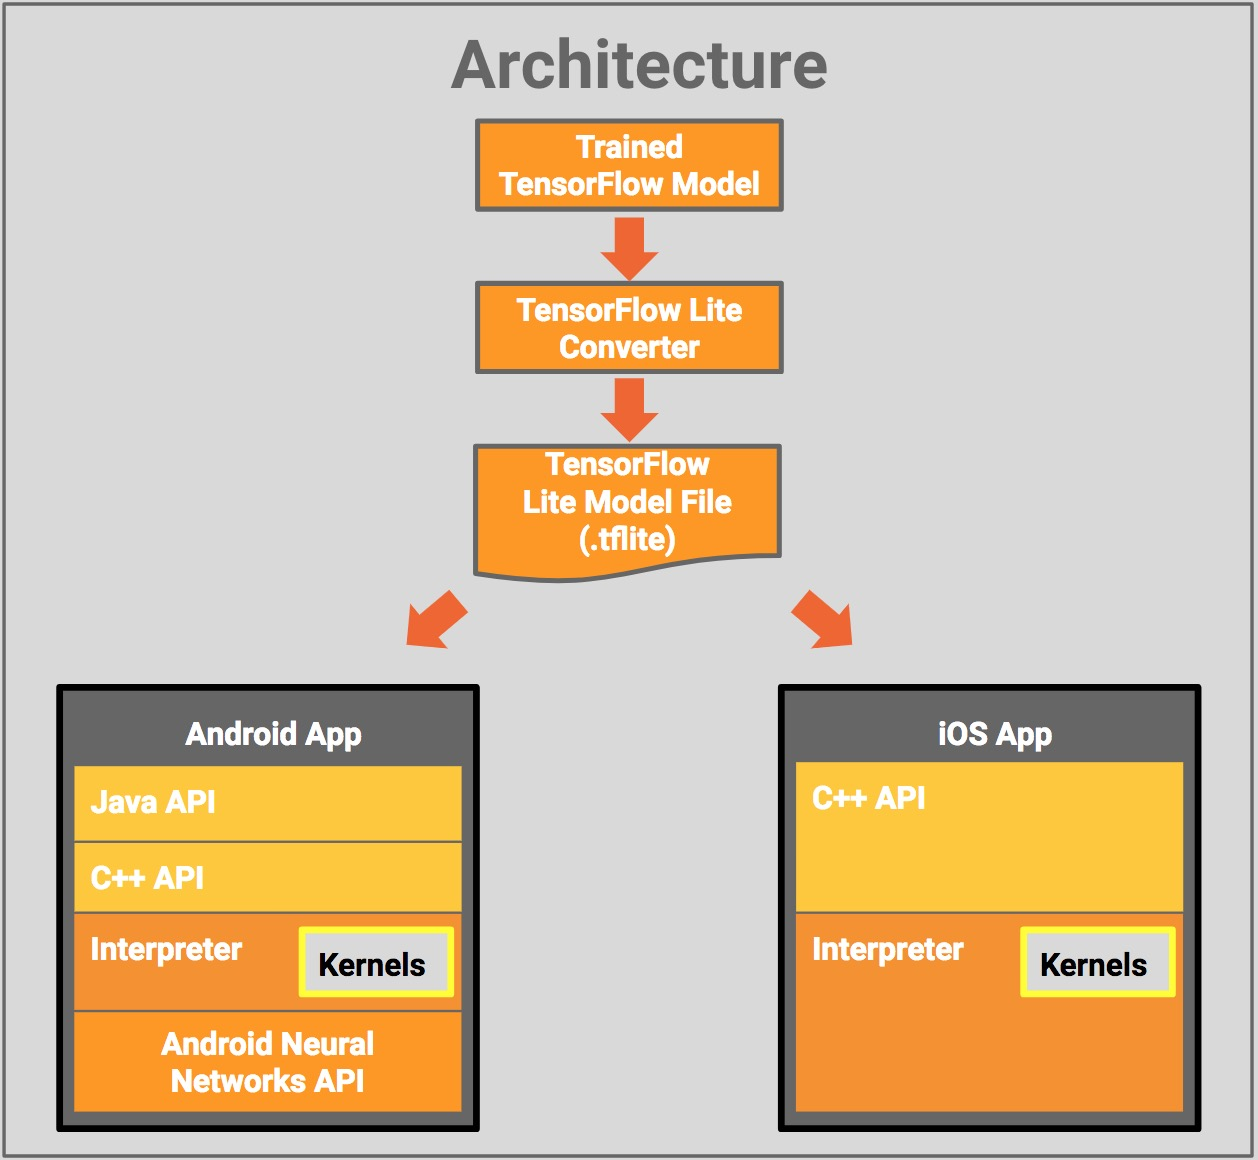
\includegraphics[scale=0.3]{tflite-architecture.jpg}
\caption{TensorFlow Lite 架构}
\end{figure}
在磁盘上开始一个训练的模型,你将用TensorFlow Lite转化器转化模型为TensorFlow Lite文件格式(.tflite)。然后你可以用转化的文件在你的移动应用上。
部署TensorFlow Lite模型文件:
\begin{itemize}
\item Java API:一个方便的在Android上围绕C++ API的包装器
\item C++ API:载入TEnsorFlow Lite模型文件,调用解释器,相同的库在Android和IOS上都可用
\item 解释器:用一些可信执行模型。解释器支持选择核心载入;没有核心仅仅100KB,3,全部载入核心300KB。这是从TensorFlow Mobile要求的1.5M重要的减小
\item 在选择的Android设备上,解释器讲用Android Neural Network API用于硬件加速,或者如果没有可用的默认使用CPU执行。
\end{itemize}
你可以用C++ API实现用于解释器的自定义核心。
\subsection{将来的工作}
在将来的版本中TensorFlow Lite讲支持更多的模型和内建操作,包括用于对固定点和浮点模型的运行改进,和让开发者更容易的开发工作刘和对其它更小的设备的支持等等。正如我们继续开发,我们希望TensorFlow Lite将简化开发者对于小型设备的开发者经历。

将来几哈用指定的机器学习硬件获取更好的可能性能用于类似设备上的类似模型。
\subsection{下一步}
对于开发者预览,多数文档在GitHub上。请查看\href{https://github.com/tensorflow/tensorflow/tree/master/tensorflow/contrib/lite}{TensorFlow Lite repository}获取更多信息和代码样例,事例应用和更多。


